\documentclass[11pt]{article}

\usepackage[margin=1in]{geometry}
\usepackage{amsmath,amssymb}
\usepackage{booktabs}
\usepackage{tabularx}
\usepackage{array}
\usepackage{graphicx}
\usepackage{xcolor}
\usepackage{microtype}
\usepackage{hyperref}
\usepackage{caption}
\usepackage{float}

\hypersetup{
    colorlinks=true,
    linkcolor=blue!55!black,
    urlcolor=blue!55!black,
    pdftitle={A/B Testing and Causal Inference: Synthesis of Notebooks 1--6},
    pdfauthor={Prepared from the Hillstrom analysis notebooks}
}

\graphicspath{{reports/figures/}{figures/}}
\setlength{\parindent}{0pt}
\setlength{\parskip}{0.55em}
\renewcommand{\arraystretch}{1.15}

\newcommand{\pp}{\,pp}
\newcommand{\emailM}{Men's Email}
\newcommand{\emailW}{Women's Email}
\newcommand{\control}{No Email}

\title{\textbf{A/B Testing and Causal Inference}\\
\large A Synthesis of Notebooks 1--6}
\author{Hillstrom Email Marketing Experiment}
\date{21 September 2026}

\begin{document}

\maketitle

\begin{abstract}
This report synthesizes six notebooks that form an end-to-end analysis of the Hillstrom email marketing experiment. The data contain 64,000 customers randomly allocated to a men's merchandise email, a women's merchandise email, or no email. The workflow validates the experiment, estimates treatment effects on visits, conversions, and spend, studies statistical power, tests treatment-effect heterogeneity, evaluates CUPED variance reduction, and demonstrates propensity-score adjustment after artificial selection bias is introduced. The randomized evidence supports both email campaigns, with the Men's Email producing the largest lift on all three outcomes. The segmentation analysis does not justify subgroup-specific targeting, and the available pre-treatment covariates provide less than 1\% variance reduction. In the observational simulation, inverse probability weighting and doubly robust estimation substantially reduce the bias of naive comparisons but do not reproduce the randomized benchmark exactly.
\end{abstract}

\begingroup
\small
\setlength{\parskip}{0pt}
\tableofcontents
\endgroup
\newpage

\section{Study Design and Analytical Scope}

The Hillstrom data record customer characteristics before treatment and three outcomes during the two weeks after treatment. Customers were assigned to one of three arms: \texttt{Mens E-Mail}, \texttt{Womens E-Mail}, or \texttt{No E-Mail}. The primary business question is whether promotional email increases site visits, purchases, and customer spend, and whether one creative performs better than the other.

Let $Y_i(a)$ denote the potential outcome for customer $i$ under campaign arm $a$. For a pair of arms $a$ and $b$, the target estimand in the randomized analysis is the intention-to-treat average effect
\begin{equation}
    \tau_{a,b}=\mathbb{E}\!\left[Y_i(a)-Y_i(b)\right].
\end{equation}
Random assignment identifies this effect by the difference in observed arm means. For binary outcomes, that difference is expressed in percentage points; for spend, it is expressed in dollars per assigned customer, including customers who spend zero.

The pre-treatment variables are recency, historical spend, purchase-history segment, product affinity, geography, new-customer status, and prior purchase channel. The outcomes are:
\begin{itemize}
    \item \textbf{Visit}: whether the customer visited the website;
    \item \textbf{Conversion}: whether the customer purchased;
    \item \textbf{Spend}: total dollars spent during the two-week observation window.
\end{itemize}

\section{Notebook 1: Dataset Validation}

Notebook 1 establishes whether the data are suitable for causal analysis. The file contains 64,000 complete observations and 12 variables. There are no missing values, no cases in which conversion occurs without a visit, and no positive-spend cases without conversion. Exact row profiles are repeated because the public file contains no customer identifier and many variables are coarse or binary. In total, 7,634 rows belong to a repeated profile (6,562 repetitions beyond the first instance). These records are retained because equality on the observed fields does not establish that they are duplicate customers.

\subsection{Randomization checks}

The observed arm sizes are extremely close to the planned 1:1:1 allocation. A Pearson sample-ratio-mismatch test gives $\chi^2=0.2025$ and $p=0.9037$, so the observed allocation is compatible with chance variation.

\begin{table}[H]
\centering
\caption{Arm sizes and observed post-treatment outcomes.}
\label{tab:arm-summary}
\begin{tabular}{lrrrr}
\toprule
Arm & $n$ & Visit rate & Conversion rate & Mean spend \\
\midrule
\emailM & 21,307 & 18.276\% & 1.253\% & \$1.423 \\
\control & 21,306 & 10.617\% & 0.573\% & \$0.653 \\
\emailW & 21,387 & 15.140\% & 0.884\% & \$1.077 \\
\bottomrule
\end{tabular}
\end{table}

Balance is also strong. Across recency, history, new-customer status, and the two product-affinity indicators, every absolute standardized mean difference between an email arm and control is below 0.009, far below the conventional 0.10 diagnostic threshold. Channel and geography proportions are similarly close across arms. Taken together, the SRM and balance checks support the randomized design, although no diagnostic can prove that every implementation detail was correct.

\subsection{Outcome distribution}

Spend is highly zero-inflated and right-skewed: 99.097\% of customers spend zero, only 578 customers have positive spend, the median is \$0, the mean is \$1.051, the standard deviation is \$15.036, and the maximum is \$499. This distribution motivates Welch standard errors, sensitivity analysis for extreme purchases, and cautious interpretation of normal-theory approximations.

\section{Notebook 2: Hypothesis Testing and Campaign Evaluation}

Notebook 2 compares all three arm pairs on all three outcomes. Visit and conversion are evaluated with two-proportion $z$-tests. Spend is evaluated with Welch's unequal-variance $t$-test. The family contains nine tests, so Benjamini--Hochberg adjustment is applied to control the false discovery rate. All nine adjusted tests reject the null at the 5\% level.

\begin{table}[H]
\centering
\caption{Pairwise treatment-effect estimates. Positive values favor the first arm.}
\label{tab:treatment-effects}
\small
\resizebox{\textwidth}{!}{%
\begin{tabular}{llllr}
\toprule
Outcome & Comparison & Estimated effect & 95\% confidence interval & BH-adjusted $p$ \\
\midrule
Visit & \emailM{} vs. \control & $7.659\pp$ & $[7.00,\ 8.32]\pp$ & $5.12\times10^{-111}$ \\
Visit & \emailW{} vs. \control & $4.523\pp$ & $[3.89,\ 5.16]\pp$ & $1.43\times10^{-43}$ \\
Visit & \emailM{} vs. \emailW & $3.136\pp$ & $[2.43,\ 3.84]\pp$ & $1.14\times10^{-17}$ \\
\addlinespace
Conversion & \emailM{} vs. \control & $0.681\pp$ & $[0.50,\ 0.86]\pp$ & $3.43\times10^{-13}$ \\
Conversion & \emailW{} vs. \control & $0.311\pp$ & $[0.15,\ 0.47]\pp$ & $2.36\times10^{-4}$ \\
Conversion & \emailM{} vs. \emailW & $0.369\pp$ & $[0.17,\ 0.56]\pp$ & $2.64\times10^{-4}$ \\
\addlinespace
Spend & \emailM{} vs. \control & \$0.770 & $[\$0.485,\ \$1.055]$ & $2.09\times10^{-7}$ \\
Spend & \emailW{} vs. \control & \$0.424 & $[\$0.169,\ \$0.680]$ & $1.27\times10^{-3}$ \\
Spend & \emailM{} vs. \emailW & \$0.345 & $[\$0.033,\ \$0.658]$ & $3.05\times10^{-2}$ \\
\bottomrule
\end{tabular}
}
\end{table}

The spend effects are small relative to customer-level dispersion: Cohen's $d$ ranges from 0.021 to 0.051. Nevertheless, the mean effect is operationally relevant because it applies across a large customer base. Per 10,000 customers, the Men's Email is estimated to generate 766 additional visits (95\% CI: 700 to 832), 68 additional conversions (95\% CI: 50 to 86), and \$7,698 additional spend (95\% CI: \$4,851 to \$10,545) relative to no email.

Winsorizing spend at the 99.9th percentile reduces the Men's-versus-control estimate from \$0.770 to \$0.659 and the Men's-versus-Women's estimate from \$0.345 to \$0.276. The signs and individual significance conclusions remain unchanged. Thus, large purchases affect the estimated magnitude but do not explain the qualitative campaign ranking. Winsorization should still be treated as a change to the outcome definition, not merely as a free precision improvement.

\section{Notebook 3: Power Analysis}

Notebook 3 asks what true effects the current design can detect with 80\% power at a two-sided 5\% significance level. For an estimated standard error $SE$, the planning approximation is
\begin{equation}
    \operatorname{MDE}\approx (z_{0.975}+z_{0.80})SE \approx 2.80SE.
\end{equation}
The resulting MDEs are planning quantities based on observed baselines and variances; they are not estimates of the true effect.

\begin{table}[H]
\centering
\caption{Minimum detectable effects at 80\% power. Relative lifts use the second arm as the baseline.}
\label{tab:mde}
\scriptsize
\begin{tabular}{lrrrrrr}
\toprule
Comparison & Visit MDE & Relative & Conversion MDE & Relative & Spend MDE & Relative \\
\midrule
\emailM{} vs. \control & $0.95\pp$ & 8.9\% & $0.26\pp$ & 45.0\% & \$0.407 & 62.3\% \\
\emailW{} vs. \control & $0.91\pp$ & 8.5\% & $0.23\pp$ & 40.2\% & \$0.365 & 55.9\% \\
\emailM{} vs. \emailW & $1.01\pp$ & 6.7\% & $0.28\pp$ & 31.5\% & \$0.447 & 41.5\% \\
\bottomrule
\end{tabular}
\end{table}

With about 21,000 customers per arm, the experiment can detect roughly a one-percentage-point visit effect, but the low conversion baseline makes even a small absolute MDE a large relative lift. Spend is the least statistically efficient outcome because of its extreme zero inflation and right tail. Winsorization reduces spend MDEs by about 19--21\%; for the Men's-versus-control comparison, the MDE falls from approximately \$0.41 to \$0.32.

Required sample size grows approximately with the inverse square of the target effect,
\begin{equation}
    n \propto \frac{1}{\operatorname{MDE}^2}.
\end{equation}
For example, detecting a 0.5-percentage-point visit effect in the Men's-versus-control comparison would require roughly 76,600 customers per arm, compared with about 21,000 currently. Halving the target MDE therefore requires approximately four times the sample.

\section{Notebook 4: Segmentation and Heterogeneous Effects}

Notebook 4 restricts attention to the Men's Email versus No Email comparison and examines effects within pre-specified groups based on recency, prior spend, channel, geography, product affinity, and customer tenure. Subgroup means and 95\% confidence intervals are descriptive. Formal heterogeneity is tested with treatment-by-segment interaction terms in OLS models with HC3 robust standard errors, followed by Benjamini--Hochberg adjustment across 30 interactions.

The estimated effects are positive across the examined subgroups, and some point estimates appear larger for selected groups, such as customers with high prior spend. However, no interaction remains significant after adjustment; the smallest adjusted $p$-value is 0.406. The correct conclusion is therefore not that every subgroup effect is identical, but that the data do not provide reliable evidence of systematic heterogeneity.

\begin{figure}[p]
    \centering
    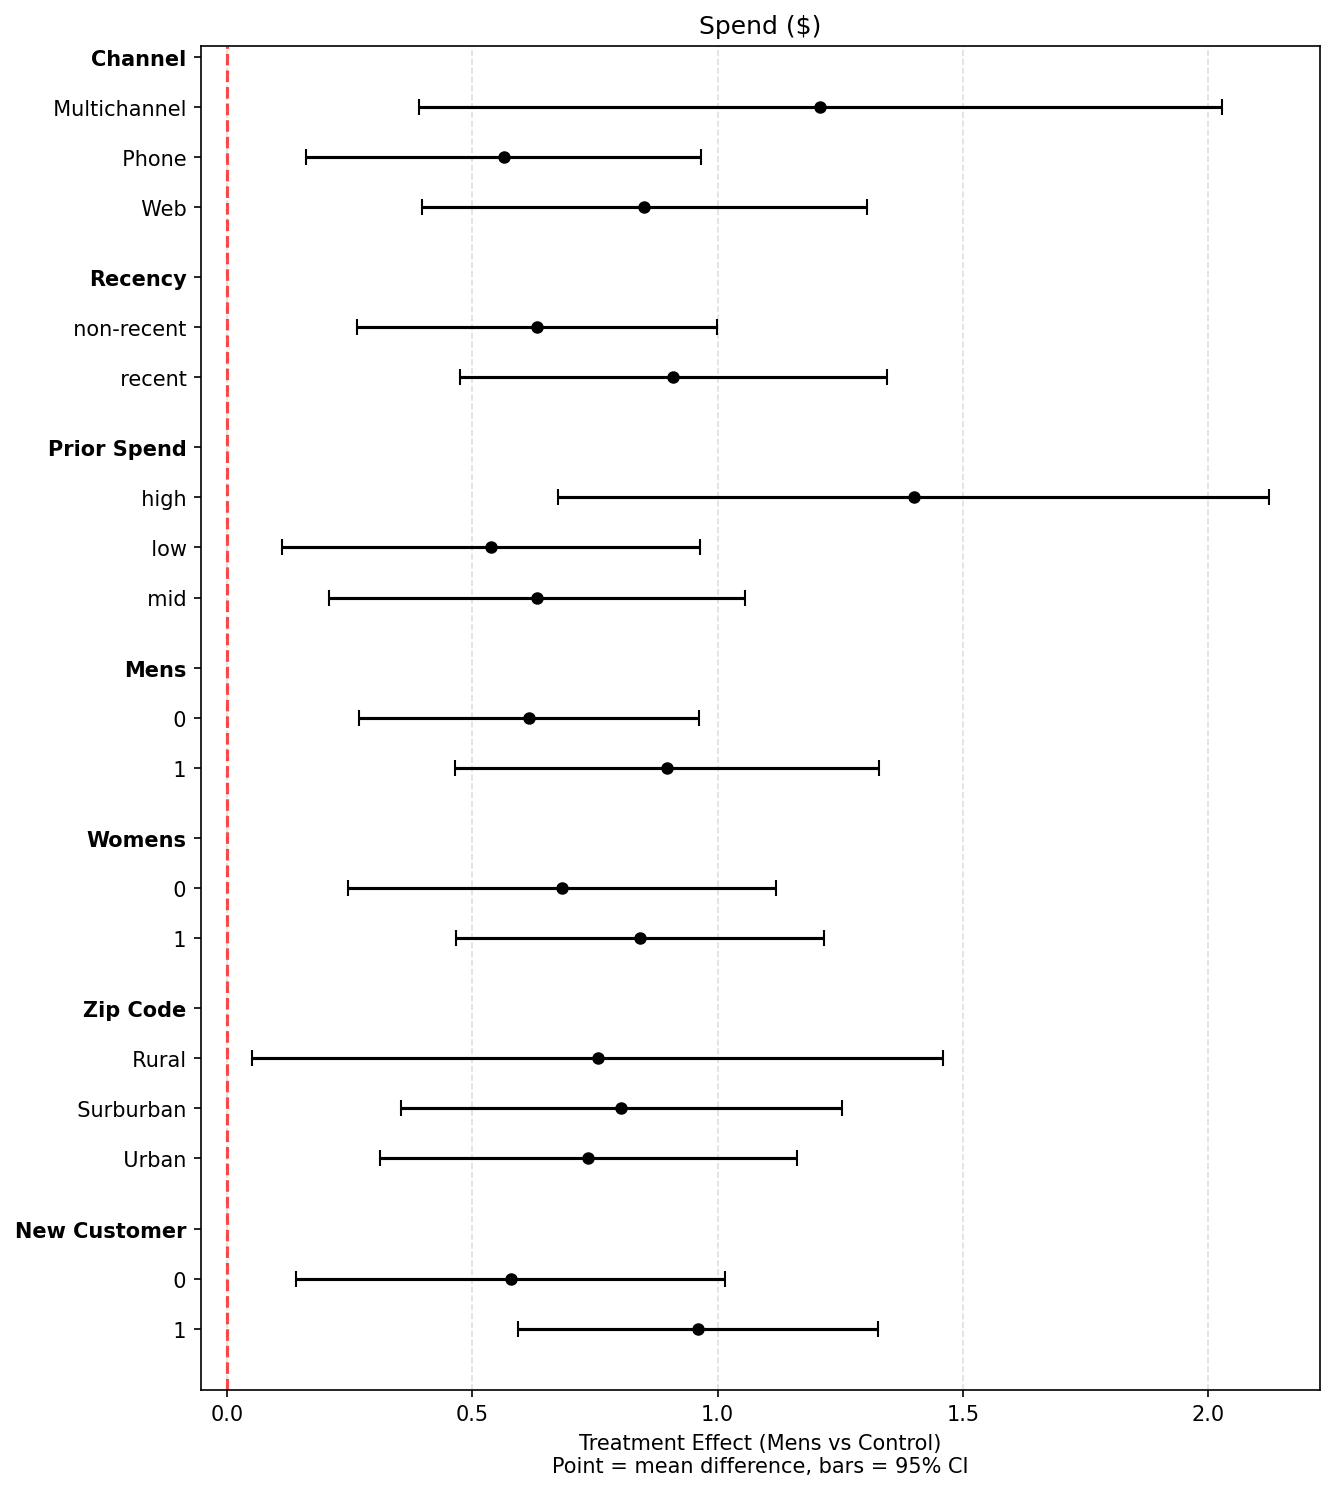
\includegraphics[width=\textwidth,height=0.82\textheight,keepaspectratio]{forest_plot_spend.png}
    \caption{Descriptive Men's Email versus No Email effects on spend across customer subgroups. The intervals summarize within-subgroup uncertainty; the formal multiplicity-adjusted interaction tests provide no evidence of heterogeneous treatment effects.}
    \label{fig:forest-spend}
\end{figure}

The practical implication is to prefer a broad rollout over segment-specific targeting. Selecting only the subgroups with the largest observed point estimates would capitalize on sampling noise. If targeting is operationally necessary, the apparent subgroup differences should be treated as hypotheses for a new experiment explicitly powered for interactions.

\section{Notebook 5: CUPED Variance Reduction}

Notebook 5 evaluates whether pre-treatment variables can improve precision for the Men's Email versus No Email estimand. For one covariate $X$, CUPED constructs
\begin{equation}
    Y_{\mathrm{CUPED}}=Y-\theta(X-\bar X), \qquad
    \theta=\frac{\operatorname{Cov}(Y,X)}{\operatorname{Var}(X)}.
\end{equation}
Centering the covariate preserves the overall outcome mean. Under randomization, the adjustment preserves the expected intention-to-treat effect while removing predictable noise. For a single linear covariate, the theoretical variance reduction is $\rho_{Y,X}^2$, equal to the simple-regression $R^2$.

All candidate variables are weak predictors of the two-week outcomes. The best individual predictor, the categorical history segment, has $R^2=0.00684$ for visit, $0.00131$ for conversion, and $0.00075$ for spend. The notebook therefore uses the continuous and nonredundant pair \texttt{history} and \texttt{recency} for multivariate adjustment.

\begin{table}[H]
\centering
\caption{Multi-covariate CUPED performance using history and recency.}
\label{tab:cuped}
\begin{tabular}{lrrr}
\toprule
Outcome & Model $R^2$ & Variance reduction & Equivalent users saved \\
\midrule
Visit & 0.008778 & 0.878\% & 374 \\
Conversion & 0.001250 & 0.125\% & 53 \\
Spend & 0.000576 & 0.058\% & 25 \\
\bottomrule
\end{tabular}
\end{table}

The adjustment works algebraically but is operationally negligible. For spend, the raw effect is \$0.7698 with standard error 0.14525 and 95\% CI $[\$0.4851,\ \$1.0545]$; the multi-covariate estimate is \$0.7690 with standard error 0.14521 and 95\% CI $[\$0.4844,\ \$1.0536]$. Visit and conversion show similarly small changes.

After CUPED, adjusted binary outcomes are continuous analysis variables and can fall slightly outside $[0,1]$. A proportion test is therefore no longer appropriate; a mean comparison or regression with robust standard errors should be used. More useful future CUPED covariates would be outcome-aligned pre-period measurements, such as visits, conversions, and spend during a comparable earlier window.

\section{Notebook 6: Causal Inference under Selection Bias}

Notebook 6 uses the randomized Men's-versus-control effect as ground truth, then creates an observational sample by retaining all controls and retaining treated customers with probability
\begin{equation}
    \operatorname{logit}^{-1}\!\left(-0.5\,\text{recency}_{z}
    +0.5\,\text{history}_{z}\right).
\end{equation}
With random seed 42, 10,521 of the 21,307 treated customers are retained, giving 31,827 observations. The retained treated group has lower mean recency (4.737 versus 5.750 months) and higher mean history (\$308.63 versus \$240.88) than control. The corresponding pre-adjustment standardized mean differences are 0.298 and 0.239, demonstrating meaningful induced imbalance.

A logistic propensity model based on recency and history is used for one-to-one nearest-neighbor matching and inverse probability weighting (IPW). Matching reduces the two observed standardized mean differences to 0.017 and 0.021. Estimated propensity scores range from roughly 0.20 to 0.82, supporting practical overlap and avoiding highly explosive weights. The doubly robust estimator combines the same treatment model with outcome regressions.

\begin{table}[H]
\centering
\caption{Treatment-effect estimates in the selection-bias simulation. Parentheses show signed percentage error relative to the randomized benchmark.}
\label{tab:causal}
\small
\begin{tabular}{lrrr}
\toprule
Method & Visit effect & Conversion effect & Spend effect \\
\midrule
Experimental benchmark & 0.0766 & 0.0068 & \$0.7698 \\
Naive biased comparison & 0.0876 $(+14.4\%)$ & 0.0080 $(+17.0\%)$ & \$0.8610 $(+11.8\%)$ \\
Propensity-score matching & 0.0715 $(-6.7\%)$ & 0.0069 $(+2.0\%)$ & \$0.8914 $(+15.8\%)$ \\
IPW & 0.0756 $(-1.3\%)$ & 0.0065 $(-4.4\%)$ & \$0.6948 $(-9.7\%)$ \\
Doubly robust & 0.0754 $(-1.5\%)$ & 0.0065 $(-4.7\%)$ & \$0.6930 $(-10.0\%)$ \\
\bottomrule
\end{tabular}
\end{table}

No estimator is closest for every outcome. IPW is closest for visit and spend, while matching is closest for conversion. Doubly robust estimates are close to IPW. In this controlled simulation, selection is generated only from the two measured covariates, so remaining discrepancies primarily reflect finite-sample variation, imperfect matching, and model specification. In a genuine observational study, conditional exchangeability would additionally require that no important unmeasured confounder remain after adjustment.

Table~\ref{tab:causal} reports values reproduced from the current notebook code and random seed. These imply an 11.8\% naive overstatement for spend; an older 28\% statement in the project README is not consistent with the current reproducible output.

\section{Integrated Conclusions and Business Recommendation}

The six notebooks support a coherent decision:
\begin{enumerate}
    \item The experiment passes the available quality, allocation, logic, and covariate-balance checks.
    \item Both email campaigns improve visits, conversions, and spend relative to no email after correction for nine comparisons.
    \item The Men's Email is the strongest arm, outperforming the Women's Email on all three outcomes.
    \item The current sample is well powered for visit-rate changes near one percentage point, but conversion and spend require comparatively large relative effects because their baselines are low and spend is highly variable.
    \item There is no adjusted-significant evidence that the Men's Email effect differs across the examined customer segments, so the evidence favors broad deployment rather than subgroup targeting.
    \item CUPED with the available covariates yields less than 1\% variance reduction and is not a material substitute for collecting stronger pre-period outcome measures or increasing sample size.
    \item When random assignment is lost, naive estimates can be biased. Propensity-score methods reduce the induced bias, but their validity depends on overlap, measured confounders, and model quality.
\end{enumerate}

The recommended campaign is therefore the Men's Email, subject to an economic check: the estimated incremental spend must be compared with delivery costs, gross margin, substitution effects, and any longer-run customer impact. Statistical significance alone does not establish profitability.

\section{Limitations}

\begin{itemize}
    \item \textbf{Short horizon.} Outcomes are measured for only two weeks, so delayed purchases and long-run customer effects are not captured.
    \item \textbf{Selected population.} The sample contains customers who purchased during the preceding year; conclusions may not generalize to lapsed customers or acquisition campaigns.
    \item \textbf{Correlated outcomes.} Visit, conversion, and spend are behaviorally nested. Benjamini--Hochberg is a reasonable multiplicity correction, but a production experiment should designate a primary overall evaluation criterion in advance.
    \item \textbf{Spend distribution.} Welch inference is robust in large samples, yet extreme zero inflation and a heavy right tail make finite-sample normal approximations and mean-based planning imperfect.
    \item \textbf{Exploratory subgroups.} Failure to reject interaction nulls is not proof of equal effects; subgroup tests can have low power even when the overall experiment is well powered.
    \item \textbf{Observational demonstration.} The selection-bias exercise is a controlled simulation, not evidence that propensity adjustment will identify effects in an arbitrary observational setting.
\end{itemize}

\appendix
\section{Notebook Map}

\begin{table}[H]
\centering
\caption{Role of each notebook in the analytical workflow.}
\begin{tabularx}{\textwidth}{@{}l>{\raggedright\arraybackslash}X@{}}
\toprule
Notebook & Main contribution \\
\midrule
01 & Validates schema, logical consistency, allocation, covariate balance, and spend distribution. \\
02 & Estimates all pairwise campaign effects, corrects nine tests, performs spend sensitivity analysis, and converts effects into business units. \\
03 & Quantifies MDEs, power curves, sample-size trade-offs, and the effect of spend winsorization on statistical sensitivity. \\
04 & Estimates subgroup effects and tests treatment-by-segment interactions with robust standard errors and multiplicity correction. \\
05 & Implements single- and multi-covariate CUPED, measures variance reduction, and compares adjusted with unadjusted inference. \\
06 & Introduces known selection bias and compares naive, matching, IPW, and doubly robust estimates with the randomized benchmark. \\
\bottomrule
\end{tabularx}
\end{table}

\end{document}
